\documentclass{beamer}
\usetheme{Berkeley} % Wybór motywu
\usecolortheme{dove} % Wybór schematu kolorów

% Informacje tytułowe
\title{Zadanie 2 stepik prezentacja}
\author{Łukasz Kulpaczyński}
\date{\today}
\usepackage[utf8]{inputenc} % kodowanie wejściowe, UTF-8
\usepackage[T1]{fontenc}    % kodowanie czcionki, obsługuje większość znaków europejskich
\usepackage[polish]{babel}  % opcjonalnie, dla lepszej obsługi języka polskiego
\usepackage{graphicx}       % do wstawiania grafik
\usepackage{amsmath}        % do trybu matematycznego
\usepackage{hyperref}       % do odnośników
\begin{document}

\frame{\titlepage} % Strona tytułowa

\begin{frame}
\frametitle{Spis treści}
\tableofcontents
\end{frame}

% Slajdy z treścią
\section{Sekcja z super zdjęciami}
\begin{frame}
\frametitle{Slajd 1}
Lorem ipsum dolor sit amet, consectetur adipiscing elit. Vivamus luctus congue tellus et lobortis. Donec sed ipsum purus. Ut nunc risus, congue et urna non, vulputate eleifend urna. Praesent egestas ipsum eu orci tincidunt laoreet. Vestibulum quis viverra sem, vel fermentum felis. Phasellus nulla felis, sollicitudin vitae orci et, imperdiet iaculis mi. Cras sit amet elementum nunc. Duis enim mi, bibendum eu imperdiet a, convallis vel est. Etiam facilisis tristique sem, sed ullamcorper velit ultricies at.
\end{frame}

\begin{frame}
\frametitle{Obraz}
\begin{figure}
\centering
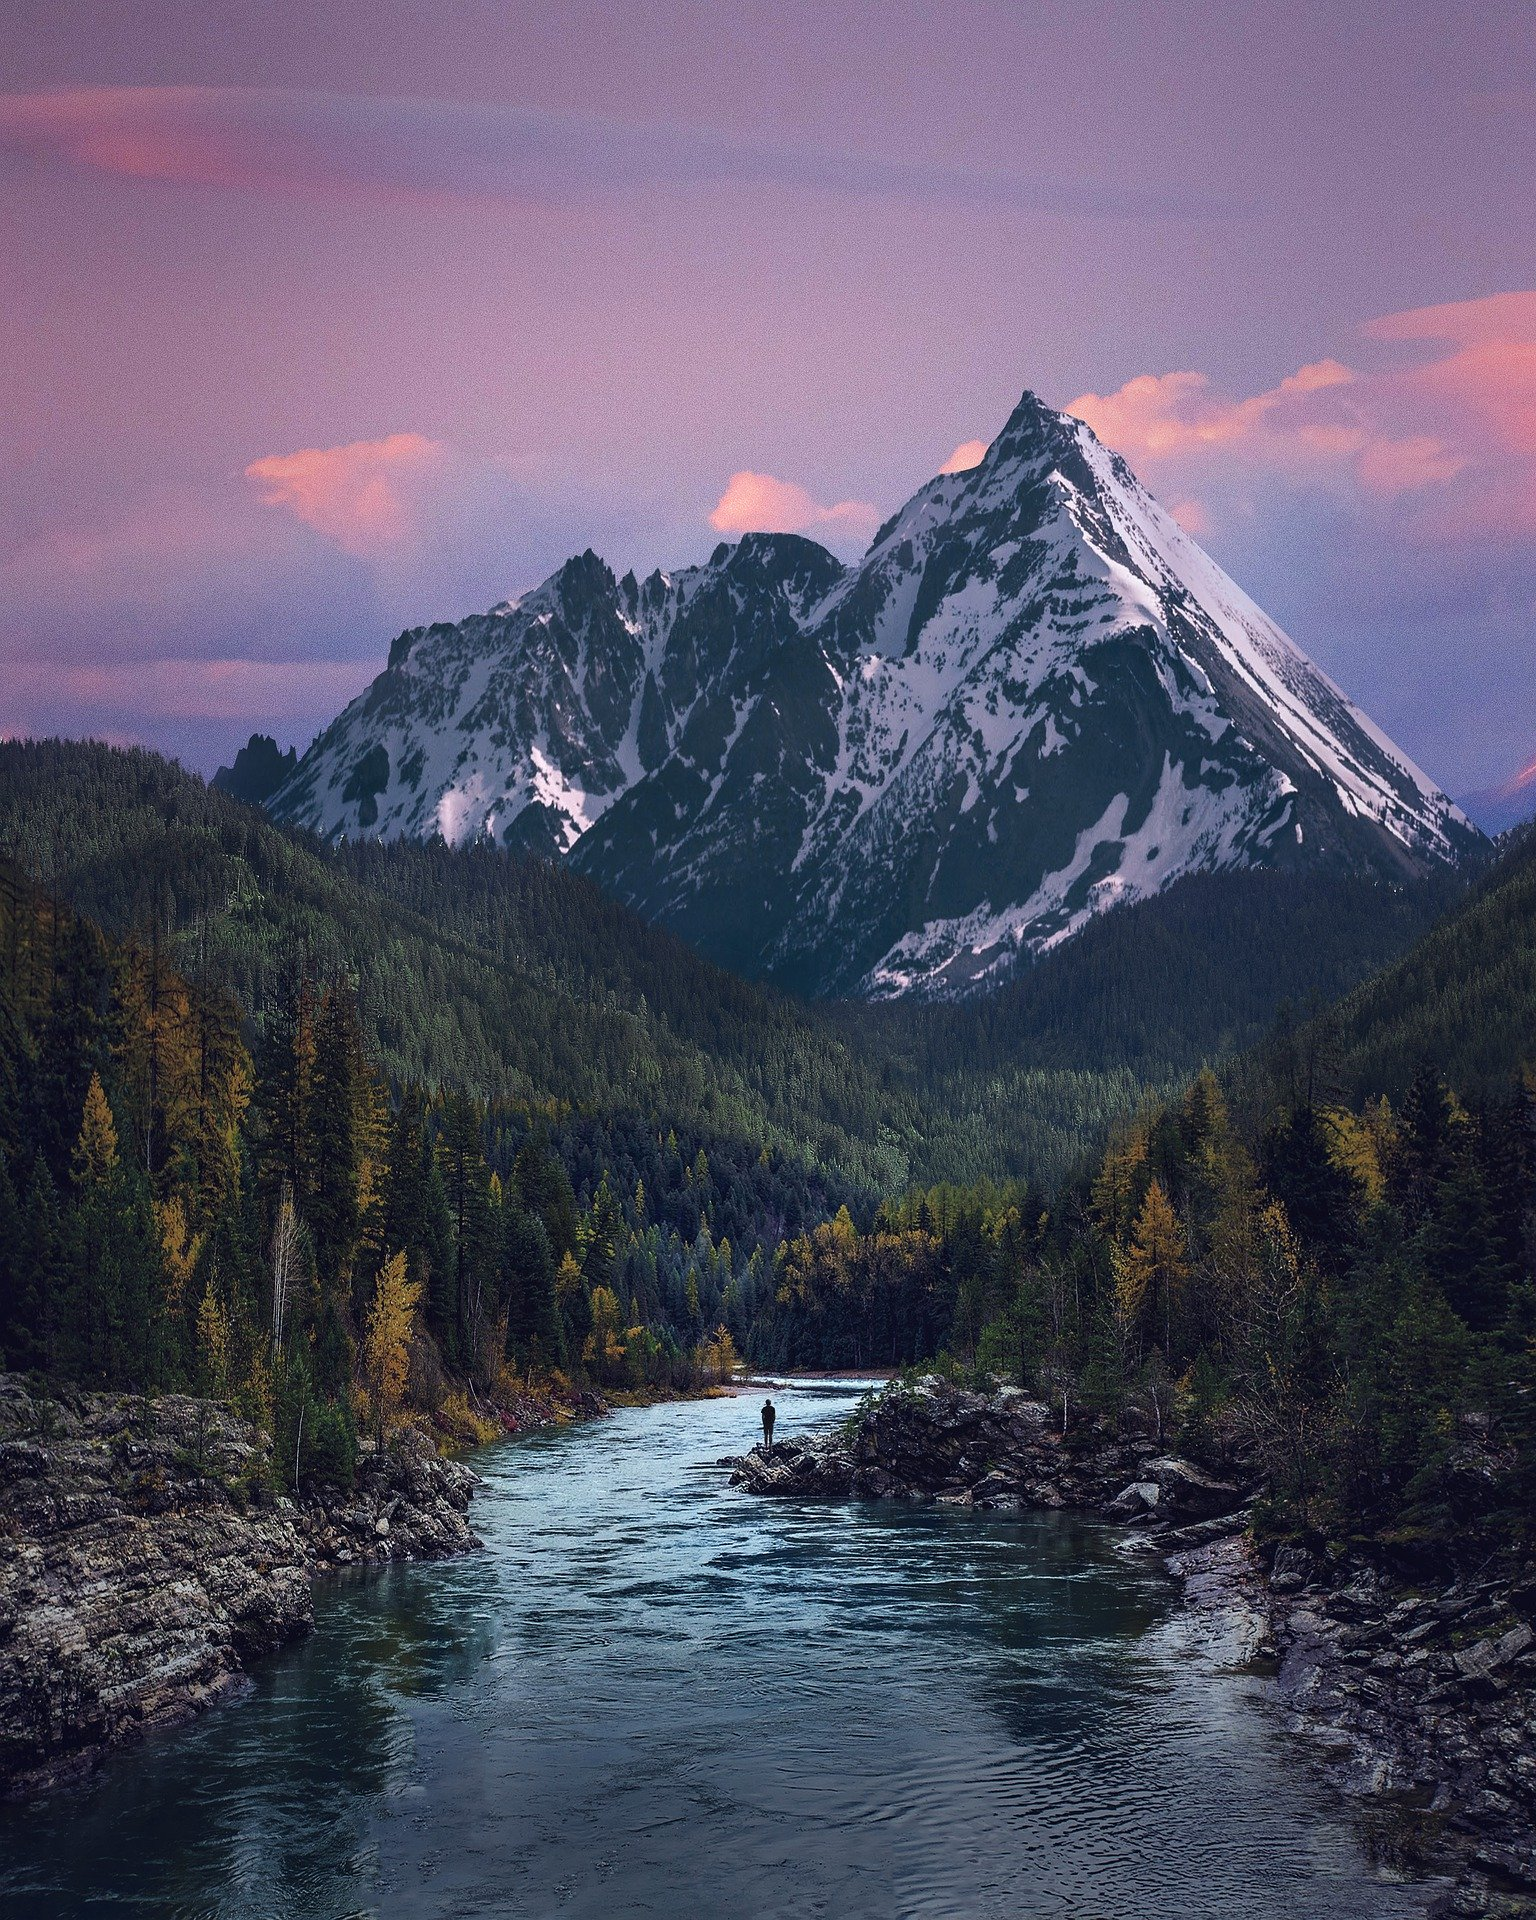
\includegraphics[width=0.5\textwidth]{valley.jpg}
\caption{Opis grafiki}
\label{fig:grafika2}
\end{figure}
\end{frame}


% Slajd z obrazkiem po lewej
\begin{frame}
\frametitle{Slajd 3}
\begin{minipage}{0.5\textwidth}
  
\includegraphics[width=\linewidth]{sponge.png}
\end{minipage}%
\begin{minipage}{0.5\textwidth}
  Spongebob once said: Lorem ipsum dolor sit amet, consectetur adipiscing elit. Vivamus luctus congue tellus et lobortis. Donec sed ipsum purus. 
\end{minipage}
\end{frame}

% Slajd z obrazkiem na środku
\begin{frame}
\frametitle{Slajd 4}
\begin{minipage}{0.5\textwidth}
  To jest ludzik lego. Donec pulvinar dolor eu felis mollis placerat. Aliquam vestibulum sed risus ultricies lacinia. In elit leo, bibendum vel mi sed, commodo auctor nisi. 
\end{minipage}%
\begin{minipage}{0.5\textwidth}
  
\includegraphics[width=\linewidth]{lego.jpeg}
\end{minipage}
\end{frame}

% Slajd z obrazkiem po prawej
\begin{frame}
\frametitle{Slajd 5}
\begin{minipage}{0.5\textwidth}
  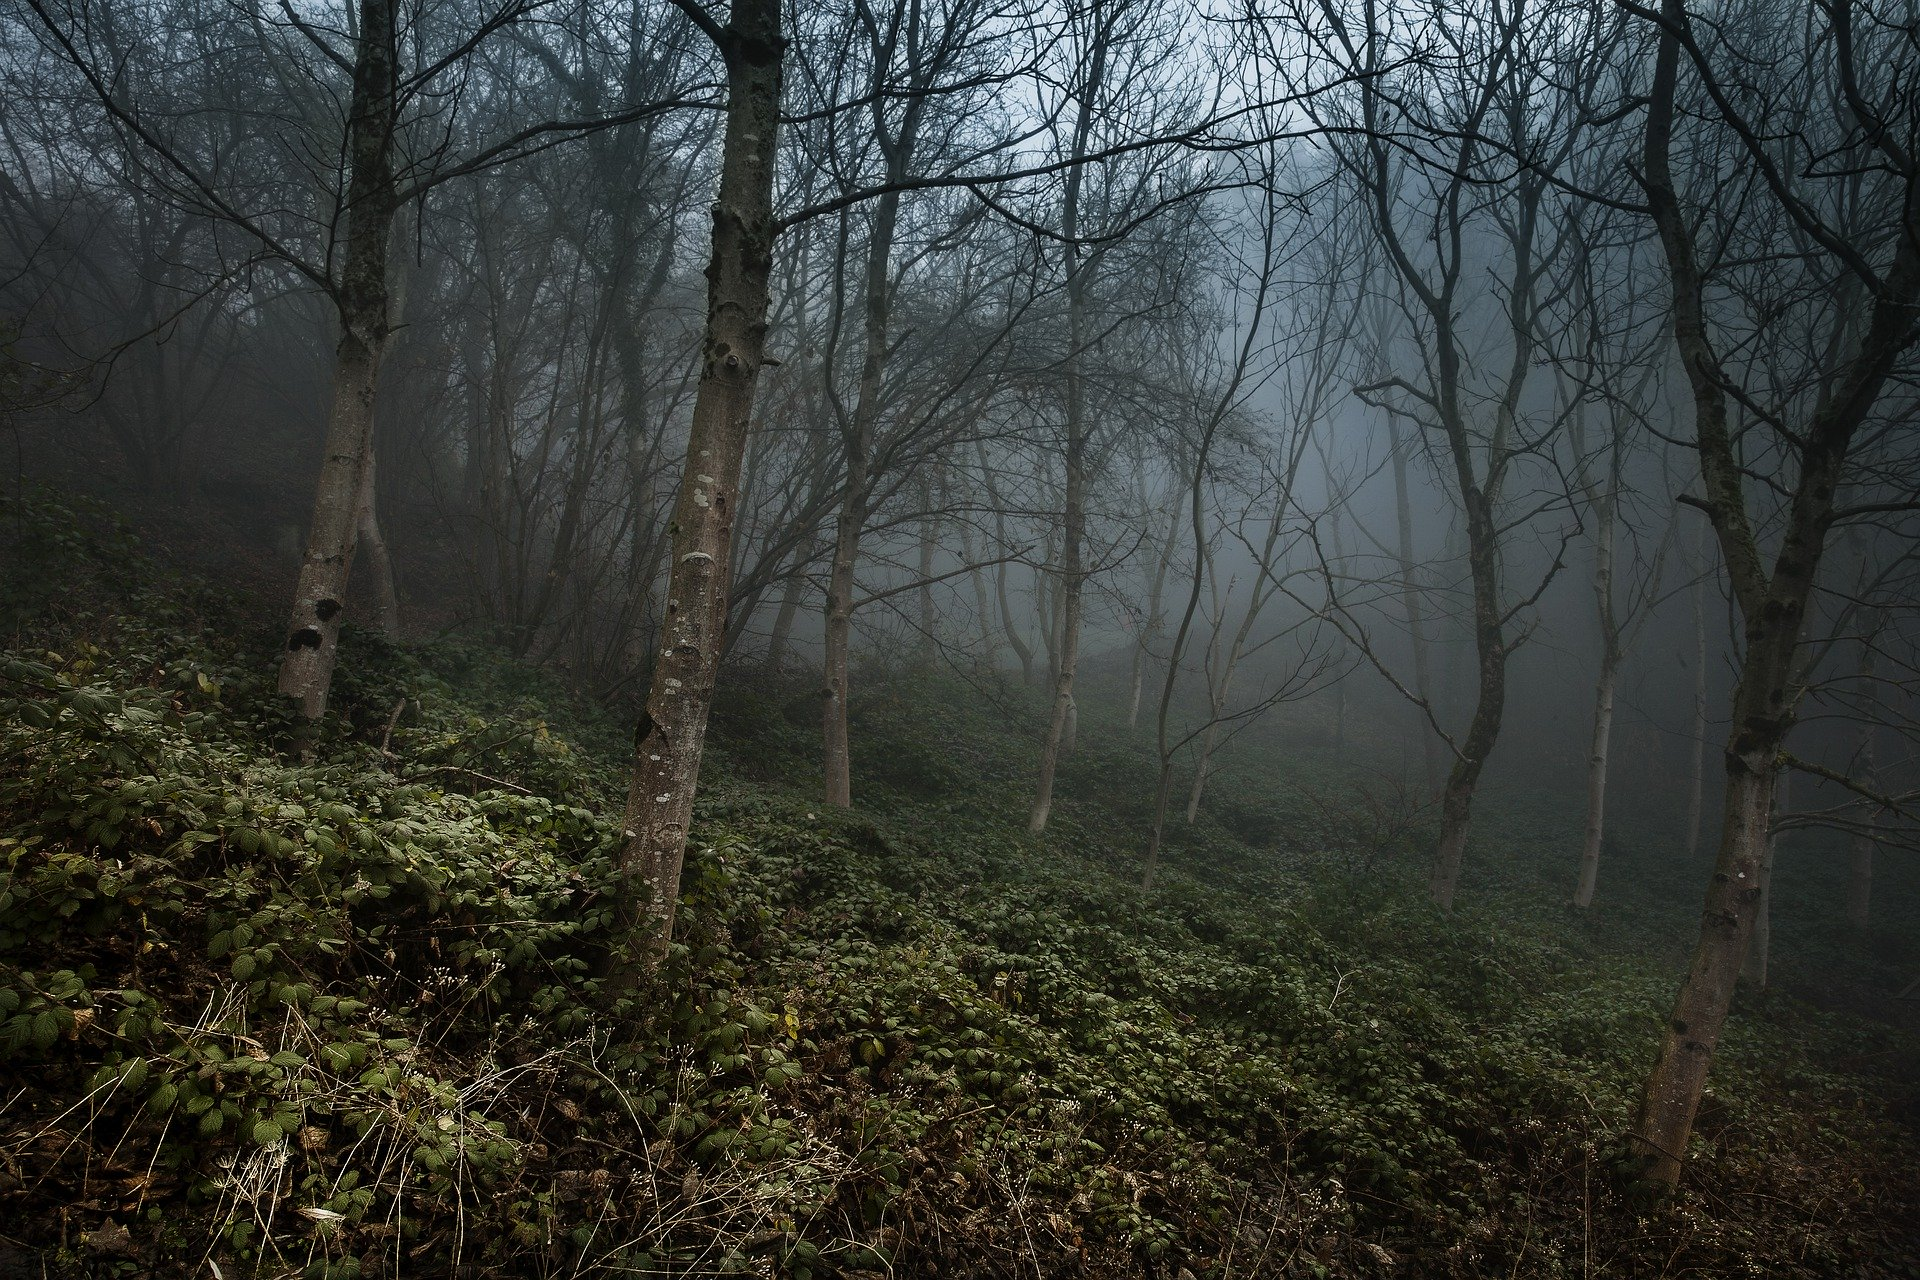
\includegraphics[width=\linewidth]{foggy.jpg}
\end{minipage}%
\begin{minipage}{0.5\textwidth}
  Duis eget purus sed diam mollis dignissim eget eget quam. Sed nec est placerat, bibendum nibh sed, ultricies ipsum. Morbi pharetra nisi ut lectus dapibus posuere.
\end{minipage}
\end{frame}

\section{Sekcja z świetną tabelą}
\begin{frame}
\frametitle{Tabela}
% Przykład wstawienia tabeli
\begin{table}
\begin{tabular}{|c|c|}
\hline
Nagłówek 1 & Nagłówek 2 \\
\hline
Wiersz 1 & Wiersz 2 \\
\hline
\end{tabular}
\caption{Przykładowa tabela}
\end{table}
\end{frame}
% Slajd z listą wypunktowaną
\begin{frame}
\frametitle{Lista 1}
\begin{itemize}
    \item Punkt pierwszy
    \item Punkt drugi
    \item Punkt trzeci
\end{itemize}
\end{frame}

% Slajd z listą ponumerowaną
\begin{frame}
\frametitle{Lista 2}
\begin{enumerate}
    \item Pierwszy element
    \item Drugi element
    \item Trzeci element
\end{enumerate}
\end{frame}

% Slajd z mieszaniem list wypunktowanych i ponumerowanych
\begin{frame}
\frametitle{Lista 3}
\begin{itemize}
    \item Główny punkt
    \begin{enumerate}
        \item Podpunkt pierwszy
        \item Podpunkt drugi
    \end{enumerate}
    \item Następny główny punkt
\end{itemize}
\end{frame}

% Bibliografia
\begin{frame}[allowframebreaks]
\frametitle{Bibliografia}
\begin{thebibliography}{10}
\bibitem{bib1} Autor, \emph{Tytuł}, Wydawnictwo, Rok.
\end{thebibliography}
\end{frame}

\end{document}
